\documentclass{standalone}
\usepackage{tikz}
\usetikzlibrary{positioning,shapes.geometric}
\begin{document}
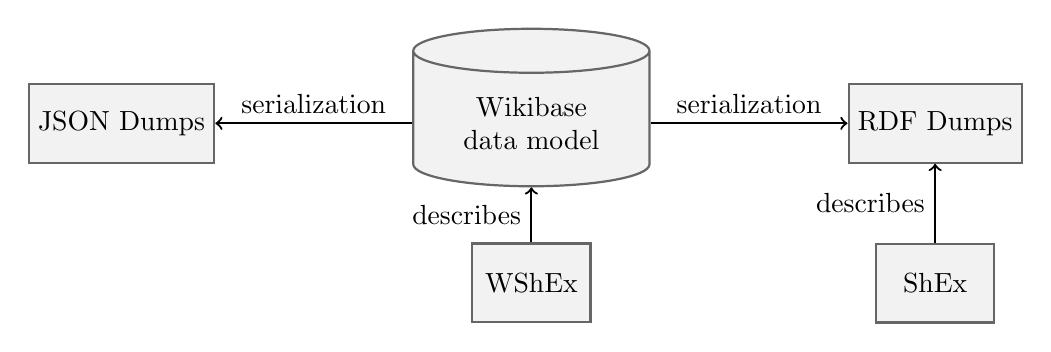
\begin{tikzpicture}[
        serialization/.style={rectangle, draw=black!60, fill=black!5, thick, minimum width=20mm, minimum height=10mm},
        schema/.style={rectangle, draw=black!60, fill=black!5, thick, minimum width=15mm, minimum height=10mm},
        db/.style={cylinder, draw=black!60, fill=black!5, thick, minimum width=30mm, minimum height = 20mm, shape border rotate=90, aspect=0.25, text width = 20mm, text centered},
    ]
    \node[db] (dataModel) {Wikibase data model};
    \node[serialization] (JSON) [left=2.5cm of dataModel] {JSON Dumps};
    \node[serialization] (RDF) [right=2.5cm of dataModel] {RDF Dumps};
    \node[schema] (ShEx) [below=1cm of RDF] {ShEx};
    \node[schema] (WShEx) [below=0.7cm of dataModel] {WShEx};

    \path[-to, thick] (dataModel.west) edge node[above] {serialization} (JSON.east);
    \path[-to, thick] (dataModel.east) edge node[above] {serialization} (RDF.west);
    \path[-to, thick] (ShEx.north) edge node[left] {describes} (RDF.south);
    \path[-to, thick] (WShEx.north) edge node[left] {describes} (dataModel.south);
\end{tikzpicture}
\end{document}